\documentclass[a4paper, dvipdfmx]{jsarticle}

\usepackage[]{../math_note, enumitem}
\usepackage{xcolor}
\usepackage{graphics}
\usepackage[all, pdf, 2cell, cmtip]{xy}
\usepackage{tikz}
\usetikzlibrary{cd, positioning, arrows}
%% for hyperref {{{
\usepackage[dvipdfmx, colorlinks=true, linkcolor=black]{hyperref}
\usepackage{pxjahyper}
%% }}}

%% environment: question/problem {{{
\usepackage{chngcntr}
\makeatletter
    \newcounter{c@question}
    \counterwithin{c@question}{section}
    \newenvironment{question}[0]%
    {\stepcounter{c@question}\begin{itembox}[l]{問\arabic{section}.\arabic{c@question}}}%
    {\end{itembox}}%
    \newenvironment{question*}[0]%
    {\stepcounter{c@question}\begin{itembox}[l]{問}}% 
    {\end{itembox}}%
\makeatother

\makeatletter
    \newcounter{c@problem}
    \counterwithin*{c@problem}{section}
    \newenvironment{problem}[0]%
    {\stepcounter{c@problem}\begin{itembox}[l]{問題\arabic{section}.\arabic{c@problem}}}%
    {\end{itembox}}%
    \newenvironment{problem*}[0]%
    {\stepcounter{c@problem}\begin{itembox}[l]{問題}}% 
    {\end{itembox}}%
\makeatother
%% }}}

\newenvironment{myenum}[1][\roman*]
{\hfill \vspace{-0.8cm}\begin{enumerate}[label=(#1), labelindent=1cm]}
{\end{enumerate}}

\newcommand{\step}[1]{\paragraph{\bf #1}}

\setenumerate{label=(\roman*),itemsep=3pt,topsep=7pt}

%% category
\newcommand{\Sch}{\mathbf{Sch}}
\newcommand{\Sets}{\mathbf{Sets}}
\newcommand{\Ring}{\mathbf{Ring}}
\newcommand{\Alg}{\mathbf{Alg}}
\newcommand{\Cat}{\mathbf{Cat}}
\newcommand{\Sh}{\mathbf{Sh}}
\newcommand{\PSh}{\mathbf{PSh}}

\newcommand{\Fib}[1]{\cat{Fib}(\cat{#1})}
\newcommand{\cFib}[1]{\cat{cFib}(\cat{#1})}
\newcommand{\sFib}[1]{\cat{sFib}(\cat{#1})}
\newcommand{\FibBP}[1]{\cat{Fib}^{\mathrm{bp}}(\cat{#1})}
\newcommand{\CFG}[1]{\cat{CFG}(\cat{#1})}
\newcommand{\Shv}[1]{\cat{Shv}(\cat{#1})}

\newcommand{\Comma}[2]{#1{\downarrow}#2}
\newcommand{\Lim}{\operatorname{lim}}
\newcommand{\Colim}{\operatorname{colim}}

\newcommand{\kiso}[1][{}]{\overset{#1}{\iso}}
\newcommand{\kequiv}[1][{}]{\overset{#1}{\simeq}}

%% derivation
\newcommand{\shDer}{\Omega}
\newcommand{\modDer}{\Omega}
\newcommand{\Der}{\mathrm{Der}}

%% functor
\newcommand{\ftor}[1]{\underline{#1}}
\newcommand{\ftorSh}{\mathit{Shff}}
\newcommand{\ftorFgt}{\mathit{Fgt}}

%% sites
\newcommand{\Cov}{\operatorname{Cov}}
\newcommand{\et}{\mathrm{et}}
\newcommand{\Et}{\mathrm{Et}}
\newcommand{\ET}{\mathrm{ET}}

%% covers
\newcommand{\covU}{\mathcal{U}}
\newcommand{\covV}{\mathcal{V}}
\newcommand{\covW}{\mathcal{W}}

%% utility
\newcommand{\mnewline}{\mbox{}\newline}
\newcommand{\tp}[2]{\texorpdfstring{#1}{#2}}
\newcommand{\parto}[2]{\mathrel{\mathop{\rightrightarrows}^{#1}_{#2}}}

%% {{{ fibered categories
\newcommand{\fib}[1]{\mathscr{#1}}
\newcommand{\fibA}{\fib{A}}
\newcommand{\fibB}{\fib{B}}
\newcommand{\fibC}{\fib{C}}
\newcommand{\fibD}{\fib{D}}
\newcommand{\fibE}{\fib{E}}
\newcommand{\fibF}{\fib{F}}
\newcommand{\fibG}{\fib{G}}
\newcommand{\fibH}{\fib{H}}
\newcommand{\fibI}{\fib{I}}
\newcommand{\fibJ}{\fib{J}}
\newcommand{\fibK}{\fib{K}}
\newcommand{\fibL}{\fib{L}}
\newcommand{\fibM}{\fib{M}}
\newcommand{\fibN}{\fib{N}}
\newcommand{\fibO}{\fib{O}}
\newcommand{\fibP}{\fib{P}}
\newcommand{\fibQ}{\fib{Q}}
\newcommand{\fibR}{\fib{R}}
\newcommand{\fibS}{\fib{S}}
\newcommand{\fibT}{\fib{T}}
\newcommand{\fibU}{\fib{U}}
\newcommand{\fibV}{\fib{V}}
\newcommand{\fibW}{\fib{W}}
\newcommand{\fibX}{\fib{X}}
\newcommand{\fibY}{\fib{Y}}
\newcommand{\fibZ}{\fib{Y}}
%% }}}

%% {{{ stacks 
\newcommand{\st}[1]{\mathcal{#1}}
\newcommand{\stA}{\st{A}}
\newcommand{\stB}{\st{B}}
\newcommand{\stC}{\st{C}}
\newcommand{\stD}{\st{D}}
\newcommand{\stE}{\st{E}}
\newcommand{\stF}{\st{F}}
\newcommand{\stG}{\st{G}}
\newcommand{\stH}{\st{H}}
\newcommand{\stI}{\st{I}}
\newcommand{\stJ}{\st{J}}
\newcommand{\stK}{\st{K}}
\newcommand{\stL}{\st{L}}
\newcommand{\stM}{\st{M}}
\newcommand{\stN}{\st{N}}
\newcommand{\stO}{\st{O}}
\newcommand{\stP}{\st{P}}
\newcommand{\stQ}{\st{Q}}
\newcommand{\stR}{\st{R}}
\newcommand{\stS}{\st{S}}
\newcommand{\stT}{\st{T}}
\newcommand{\stU}{\st{U}}
\newcommand{\stV}{\st{V}}
\newcommand{\stW}{\st{W}}
\newcommand{\stX}{\st{X}}
\newcommand{\stY}{\st{Y}}
\newcommand{\stZ}{\st{Z}}
%% }}}


\newcommand{\Diag}{\Delta}
\newcommand{\rest}{\vspace{5pt}}
\newcommand{\rep}{{\color{blue}\#}}
\newcommand{\arpb}{\ar[lu, phantom, "\text{p.b.}"]}
\newcommand{\Isom}{\cat{Isom}}

\begin{document}
\title{第5章 \\ Algebraic Stacks and Spaces}
\author{七条彰紀}
\maketitle
\tableofcontents
\vspace{10pt}

affine scheme, scheme. algebraic space, algebraic stackという貼り合わせの連なりを意識した定義をした後,
algebraic stackがschemeの貼り合わせとして定義できることを示す.
algebraic spaceとalgebraic stackの定義は全く平行に行われる.
そのことが分かりやすい記述を志向する.

\section{Fiber Product}
\begin{Prop}
    任意のsite :: $\cat{C}$について,
    $\cat{C}$上のsheafの圏$\Shv{C}$はfiber poductを持つ.
\end{Prop}
\begin{proof}
    二つの射$\shF \to \shH, \shG \to \shH$をとる.
    \[ \cat{C} \ni U \mapsto \shF(U) \times_{\shH(U)} \shG(U) \]
    とすれば,これはfiber productとなる.
\end{proof}

$\cat{B}$ :: categoryとする.
この時,$\FibBP{B}$は以下のような圏であった.
\begin{description}[labelindent=1cm]
    \item[Objects:] fibered categories over $\cat{B}$.
    \item[Arrows:]  base-preserving natural transtormation.
\end{description}
新たに圏$\CFG{B}$を以下のように定義する.
\begin{description}[labelindent=1cm]
    \item[Objects:] categories fibered in groupoids(CFG) over $\cat{B}$.
    \item[Arrows:] base-preserving natural transtormation.
\end{description}

重要なのは次の存在命題である.
\begin{Prop}[\cite{Gomez99} p.10]
    任意の圏$\cat{C}$について,
    $\FibBP{B}$と$\CFG{B}$はfibered productを持つ.
\end{Prop}
%% {{{
\begin{proof}
    $\FibBP{B}$の射$F \colon \stX \to \stZ$と$F \colon \stY \to \stZ$をとり,
    $F, G$のfiber productを実際に構成する.

    \step{圏$\cat{P}$の構成}
    圏$\cat{P}$を以下のように定義する.
    \begin{description}
        \item[Objects:]
            以下の$4$つ組
            \begin{enumerate}
                \item $b \in \cat{B}$,
                \item $x \in \stX(b)$,
                \item $y \in \stY(b)$,
                \item $\stZ$の恒等射上の同型射$\alpha \colon Fx \to Gy$.
            \end{enumerate}
        
        \item[Arrows:] \mnewline
            射$(b, x, y, \alpha) \to (b', x', y', \alpha')$は,
            二つの射$\phi_{\stX} \colon x \to x', \phi_{\stY} \colon y \to y'$であって以下を満たすもの:
            $\phi_{\stX}, \phi_{\stY}$は同じ射$b' \to b$上の射で,
            以下の可換図式を満たすもの.
            \[
            \begin{tikzcd}
                Fx \ar[d, red, "F\phi_{\stX}"']\ar[r, "\alpha"]& Gy \ar[d, red, "G\phi_{\stY}"]\\
                Fx' \ar[r, "\alpha'"']& Gy'
            \end{tikzcd}
            \]
    \end{description}

    \step{Cartesian Lifting in $\cat{P}$.}
    この圏は$\pi \colon (b,x,y,\alpha) \mapsto b$によってfibered categoryと成る.
    $f \colon b' \to b$の$\xi=(b, x, y, \alpha)$に関する
    Cartesian Lifting :: $f^*\xi \to \xi$は次のように定義される.
    \[
        \chi_{\xi}=(f^*x \xrightarrow{\chi_x} x, f^*y \xrightarrow{\chi_y} y)
        \colon
        f^*\xi=(b', f^*x, f^*y, \bar{\alpha}) \to \xi.
    \]
    ここで$\chi_x \colon f^*x \to x$は$f$の$x$に関するCartesian Liftingである.
    $\chi_y$も同様.
    さらに$\bar{\alpha}$は以下のTriangle Liftingで得られる射である
    \footnote
    {
        $f^*\alpha \colon f^*Fx \to f^*Gy$とは異なる.
        同型$Ff^*x \to F^*Fx, Gf^*y \to f^*Gy$と$f^*\alpha \colon Fx \to Gy$を
        合成しても$\bar{\alpha}$は得られる.
    }.
    \begin{center}
    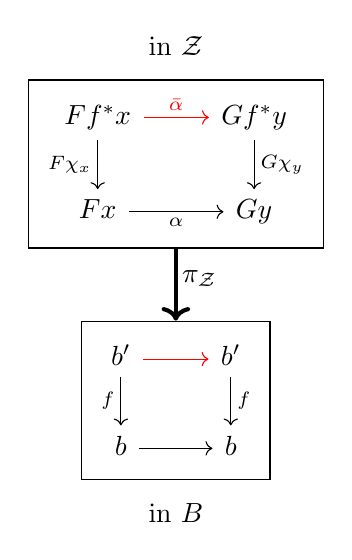
\begin{tikzpicture}[mybox/.style={draw, inner sep=5pt}]
    \node[mybox] (X) at (0,3){%
        \begin{tikzcd}
            Ff^*x \ar[d, "F\chi_x"']\ar[r, red, "\bar{\alpha}"]& Gf^*y \ar[d, "G\chi_y"]\\
            Fx \ar[r, "\alpha"']& Gy
        \end{tikzcd}
    };
    \node[mybox] (B) at (0,0){%
        \begin{tikzcd}
            b' \ar[d, "f"']\ar[r, red, "\id"]& b' \ar[d, "f"]\\
            b \ar[r, "\id"]& b
        \end{tikzcd}
    };

    \node [above=5pt of X] {in $\stZ$};
    \node [below=5pt of B] {in $\cat{B}$};
    \draw [->, line width=1.5pt] (X) edge (B);
    \node at (0.3,1.55) {$\pi_{\stZ}$};
    \end{tikzpicture}
    \end{center}
    fibered categoryの間の射はcartesian arrowを保つので$F\chi_x, G\chi_y$もcartesian.
    したがってTriangle Liftingが出来る.
    $\bar{\alpha}$が同型であることはTriangle Liftingの一意性を用いて容易に証明できる.
    また,この可換図式から$\chi_{\xi}$が$\cat{P}$の射であることも分かる.

    \step{$\stX, \stY, \stZ$がcategory fibered in groupoids(CFG)ならば$\cat{P}$もCFG}
    $\stX, \stY, \stZ$がCFGならば$\cat{P}$もCFGとなる.
    実際,
    $\phi_{\stX} \colon x \to x'$と$\phi_{\stY} \colon y \to y'$の両方がcartesianならば
    $(\phi_{\stX}, \phi_{\stY}) \colon (b, x, y, \alpha) \to (b', x', y', \alpha')$はcartesianである.

    \step{$\cat{P}$からの射影写像.}
    定義から明らかに$\pr_1 \colon \cat{P} \to \stX, \pr_2 \colon \cat{P} \to \stY$が定義できる.
    射の定義にある可換図式は,
    以下の$A$がnatural transformationであることを意味している.
    \begin{defmap}
        A \colon & F\pr_1& \to& G\pr_2 \\
        {}& (F\pr_1)((b, x, y, \alpha))=Fx& \mapsto& \alpha(Fx)=\alpha((F\pr_1)((b, x, y, \alpha)))
    \end{defmap}
    $A$がbase-preservingであることは$\alpha$が恒等射上のもの(i.e. $\pi_{\stZ}(\alpha)=\id$)であることから,
    isomorphismであることは$\alpha$が同型であることから示される.

    \step{$\cat{P}$ :: fiber product.}
    今,
    $\stW \in \FibBP{B}$と
    射$S \colon \stW \to \stX, T \colon \stW \to \stY$及び
    base-preserving isomorphism :: $\delta \colon FS \to GT$をとる.
    base-preservingなので,任意の$w \in \stW$について$\pi_{\stZ}(FS(w))=\pi_{\stZ}(GT(w))$.
    そこで次のように関手が定義できる.
    \begin{defmap}
        H\colon & \stW& \to& \cat{P} \\
        \mathbf{Object}& w& \mapsto& (\pi_{\stZ}(FS(w)), Sw, Tw, \delta_{w}) \\
        \mathbf{Arrow}& [\phi \colon w \to w']& \mapsto& (S\phi \colon Sw \to Sw', T\phi \colon Tw \to Tw')
    \end{defmap}
    このように置くと,$S=\pr_1 H, T=\pr_2 H$となる.
    逆に$S \iso \pr_1 H', T \iso \pr_2 H'$となる
    関手$H' \colon \stW \to \cat{P}$は$H$と同型に成ることが直ちに分かる.
\end{proof}
%% }}}
\begin{Remark}
    session4 命題4.5より,CFGの恒等射上の射は同型射である.
    したがって$\alpha \colon Fx \to Gy$に課せられた条件は,
    $\stZ$がCFGならば一つしか無い.
\end{Remark}

\begin{Example}
    representable fibered categoryのfiber product.
    
    sheafに対応するfibered categoryの
    fiber product $\int \shF \times_{\int \shH} \int \shG$に対応するsheafは,
    sheafのfiber productに対応する.
    \[
        \left( \int \shF \times_{\int \shH} \int \shG \right)(-)
        =\shF \times_{\shH} \shG
        \quad \in \Shv{C}
    \]
\end{Example}

我々が扱うのはstackであるから,
stackという性質がfiber productで保たれていて欲しいが,果たしてそうなる.
\begin{Prop}[\cite{Olsson16} Prop 4.6.4]
    $\stX, \stY, \stZ$ :: stack over $\cat{C}$とし,
    morphism of stacks :: $F \colon \stX \to \stZ, G \colon \stY \to \stZ$をとる.
    この時,$F, G$についてのfiber product :: $\stX \times_{\stZ} \stY$はstackである.
\end{Prop}
したがって結局$\FibBP{B}, \CFG{B}$と,
stackの圏及びstack in groupoidsの圏はfiber productを持つ.
我々が実際に扱うのはstack in groupoidsである.
%% {{{
\begin{proof}
    $\stP=\stX \times_{\stZ} \stY$とおく.
    $U \in \cat{C}, \covU=\{\phi_i \colon U_i \to U\} \in \Cov(U)$を任意にとり,
    $\epsilon_{\covU} \colon \stP(U) \to \stP(\covU)$を計算する.

    \step{$\epsilon_{\covU}(\xi)$.}
    $\xi=(b, x, y, \alpha)$をとり,$\epsilon_{\covU}(\xi)$を計算する.
    まず$\{\phi_i^*\xi\}_i$は既に詳しく説明した.
    注意が必要なのは同型$\sigma_{ij} \colon \pr_2^*\phi_i^*\xi \to \pr_1^*\phi_j^*\xi$である.
    可換性は以下の図式から分かる.
    \begin{center}
    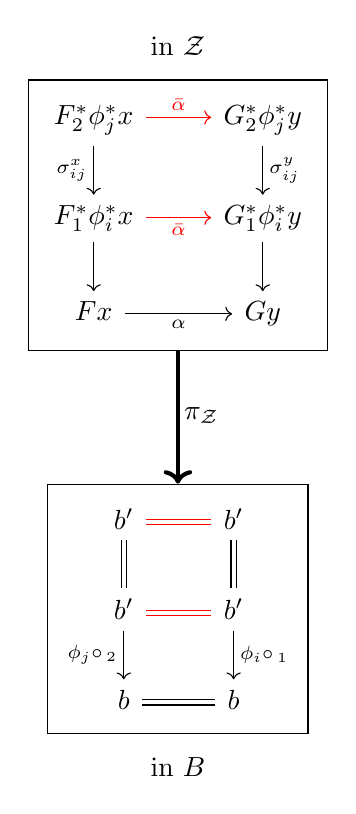
\begin{tikzpicture}[mybox/.style={draw, inner sep=5pt}]
    \node[mybox] (X) at (0,5){%
        \begin{tikzcd}
            F\pr_2^*\phi_j^*x \ar[d, "\sigma_{ij}^{x}"']\ar[r, red, "\bar{\alpha}"]&
            G\pr_2^*\phi_j^*y \ar[d, "\sigma_{ij}^{y}"]\\
            F\pr_1^*\phi_i^*x \ar[d]\ar[r, red, "\bar{\alpha}"']& G\pr_1^*\phi_i^*y \ar[d]\\
            Fx \ar[r, "\alpha"']& Gy
        \end{tikzcd}
    };
    \node[mybox] (B) at (0,0){%
        \begin{tikzcd}
            b' \ar[r, red, equal]\ar[d, equal]& b' \ar[d, equal] \\
            b' \ar[r, red, equal]\ar[d, "\phi_j \circ\, \pr_2"']& b' \ar[d, "\phi_i \circ\, \pr_1"]\\
            b \ar[r, equal]& b
        \end{tikzcd}
    };

    \node [above=5pt of X] {in $\stZ$};
    \node [below=5pt of B] {in $\cat{B}$};
    \draw [->, line width=1.5pt] (X) edge (B);
    \node at (0.3,2.45) {$\pi_{\stZ}$};
    \end{tikzpicture}
    \end{center}
    
    \step{$\epsilon_{\covU}(\kappa)$.}
    (TODO)

\end{proof}
%% }}}
\section{Diagonal Map}
\begin{Remark}
    以降は$S$ :: schemeをとり,
    $\cat{C}=\ET(S)$ :: big etale site over $S$上の
    sheafあるいはstack in groupoidsのみを考える.
\end{Remark}

\begin{Def}[Diagonal Map]
    sheafあるいはstack in groupoids over $S$:: $\stX/S$(すなわち射$\stX \to S$)
    のdiagonal map :: $\Diag$とは,
    以下の可換図式に収まる射のことである.
    \[\begin{tikzcd}
            \stX \ar[rrd, bend left, "\id"]\ar[rdd, bend right, "\id"']\ar[rd, "\Diag"]&
                                                            & \\
                                                            &
        \stX \times \stX \ar[r]\ar[d]\ar[rd, phantom, "\text{p.b.}"]& \stX \ar[d]\\
          &\stX \ar[r]& S
    \end{tikzcd}\]
\end{Def}

\section{Local Property of Scheme/Morphism of Them}
\begin{Def}[\cite{DM69} p.100, Local Property for the topology.]
    $S$ :: schemeとし,$(\Sch/S)$上のsite :: $\cat{C}$を考える.
    $X, Y$ :: schemeとし,
    $\{\phi_i \colon X_i \to X\} \in \Cov(X), \{\psi_i \colon Y_i \to Y\} \in \Cov(Y)$を任意に取る.
    \begin{enumerate}
        \item 
            $P$をschemeの性質とする.
            $P$がlocal for the topologyであるとは,以下が成り立つということ: \mnewline
            $X$が$P$であることは,全ての$U_i$が$P$であることと同値.
        \item
            $P$をschemeの射の性質とする.
            $P$がlocal on sourceであるとは,以下が成り立つということ:\mnewline
            $f \colon X \to Y$が$P$であることは,
                全ての$f \circ \phi_i$が$P$であることと同値.
        \item
            $P$をschemeの射の性質とする.
            $P$がlocal on targetであるとは,以下が成り立つということ:\mnewline
            $f \colon X \to Y$が$P$であることは,
                全ての$\pr_2 \colon X \times_Y Y_i \to Y_i$が$P$であることと同値.
        \item
            (\cite{Olsson16} 5.1.3)
            $P$をschemeの射の性質とする.
            以下が全て成り立つ時,$P$はstableであると呼ばれる.
            \begin{itemize}
                \item 任意の同型は$P$.
                \item $P$は,射の合成で保たれる.
                \item $P$は,任意の$\cat{C}$の射によるbase changeで保たれる.
                \item local on target.
            \end{itemize}

        \item
            (\cite{LMB} p.33, \cite{Gomez99} p.16)
            $P$をschemeの射の性質とする.
            以下が全て成り立つ時,
            $P$はsmooth (resp. etale) local on source and targetであると呼ばれる.:
            $X' \to Y' \times X, Y' \to Y$がsmooth (resp. etale) surjectiveであるような,
            次の形の任意の可換図式をとる.
            \[
            \begin{tikzcd}
                X' \ar[r] \ar[rd, "f'"']& Y' \times X \ar[r]\ar[d]& X \ar[d, "f"]\\
                {} & Y' \ar[r]& Y \ar[lu, phantom, "\text{p.b.}"]
            \end{tikzcd}
            \]
            この時,$f$が$P$であることは$f'$が$P$であることと同値.
    \end{enumerate}
\end{Def}

\begin{Example}[\cite{SP} Tag 0238]
    etale topologyでの定義を挙げる.
    \begin{description}
    \item[local for the topologyである性質の例] \mnewline
        locally Noetherian, reduced, normal, regular.

    \item[local on sourceである性質の例] \mnewline
        flat, locally of finite presentation, locally of finite type, open,
        smooth, etale, unramified, locally quasi-finite.

    \item[local on targetである性質の例] \mnewline
        quasi-compact, quasi-separated, universally closed, separated, surjective,
        locally of finite type, locally of finite presentation,
        proper, smooth, etale, unramified, flat.

    \item[local on source and targetである性質の例] \mnewline
        flat, locally of finite presentation, locally finite type,
        smooth, etale, unramified...
    \end{description}
\end{Example}

\begin{Remark}
    ``local on source and target"は,
    algebraic space, algebraic stackの射について性質を定めるときに必要に成る.
    この定義は文献に寄って数種類ある.
    私が知る限りのものを以下に列挙する.
    \begin{description}
        \item[SP] \mnewline
            \cite{SP} Tag 04QZ.

        \item[DM] \mnewline
            $X, Y$をschemeとし,
            $\{\phi_i \colon X_i \to X\} \in \Cov(X), \{\psi_i \colon Y_i \to Y\} \in \Cov(Y)$を任意のcoverとする.
            $\{ f_i \colon X_i \to Y_i \}$を以下の可換図式を満たす射の族とする.
            \[
            \begin{tikzcd}
                X_i \ar[r, "\phi_i"]\ar[d, "f_i"']&  X \ar[d, "f"]\\
                Y_i \ar[r, "\psi_i"']& Y
            \end{tikzcd}
            \]
            この時,射$f$が$P$であることと,全ての射$f_i$が$P$であることは同値.
            \cite{DM69}, p.100より.
        
        \item[DM'] \mnewline
            以下のschemeの可換図式が成立しているとする.
            \[
            \begin{tikzcd}
                X' \ar[r]\ar[d, "f'"']&  X \ar[d, "f"]\\
                Y' \ar[r]& Y
            \end{tikzcd}
            \]
            ただし$X' \to X, Y' \to Y$はcoverである.
            この時,射$f$が$P$であることと,射$f'$が$P$であることは同値.
            \cite{SP} Tag 04R4でDeligne-Mumfordの定義として参照されている.
        
        \item[ST] \mnewline
            local on sourceかつlocal on target.

        \item[ST+] \mnewline
            次の5条件を合わせたもの.
            \begin{itemize}
                \item 同型について成立する,
                \item stable under composition,
                \item stable under base change,
                \item local on source,
                \item local on target.
            \end{itemize}
            \cite{Olsson16} Def 5.1.3, 5.4.11で採用されている.

        \item[La] \mnewline
            $X, Y$ :: schemeとし,射$Y' \to Y, X' \to Y' \times X$をcoverとする.
            この時,$f \colon X \to Y$と合わせると次の可換図式が得られる.
            \[
            \begin{tikzcd}
                X' \ar[r] \ar[rd, "f'"']& Y' \times X \ar[r]\ar[d]& X \ar[d, "f"]\\
                {} & Y' \ar[r]& Y \ar[lu, phantom, "\text{p.b.}"]
            \end{tikzcd}
            \]
            この時,$f$が$P$であることは$f'$が$P$であることと同値.
            \cite{LMB} p.33, \cite{Gomez99} p.16で採用されている.
        
        \item[La'] \mnewline
            $X, Y$ :: schemeとし,射$Y' \to Y, X' \to X$をcoverとする.
            この時,$f \colon X \to Y$と合わせると次の可換図式が得られる.
            \[
            \begin{tikzcd}[row sep=30pt]
                X' \times_Y Y' \ar[rr]\ar[d, "f'"']& {} & Y' \ar[d]\\
                X' \ar[r]& X \ar[r, "f"']& Y \ar[llu, phantom, "\text{p.b.}"]
            \end{tikzcd}
            \]
            この時,$f$が$P$であることは$f'$が$P$であることと同値.
    \end{description}
    
    強弱関係は次の通り.
    \[
    \begin{tikzcd}[every arrow=Rightarrow]
        ST+ \ar[r, Rightarrow]& SP \ar[r, Rightarrow]&
        DM \ar[r, Rightarrow]\ar[rd, Rightarrow]& DM' \ar[r, Rightarrow]& La \ar[r, Rightarrow]& La' \\
                                                & & & ST \ar[u, Rightarrow]& &
    \end{tikzcd}
    \]
    SP$\implies$DM$\implies$STは\cite{SP} Tag 04R4による.
    SP$\implies$DM$\implies$ST, DM'$\implies$La$\implies$La'の
    それぞれの$\implies$は逆が成り立たないことも分かっている.
    また,DM'とlocal on targetを合わせたものはDMと同値である.
    
    我々としては,「便利な性質」をもち,かつ弱い定義を取りたい.
    後に示すとおり,Laを仮定すれば十分「便利」である.
\end{Remark}

\section{Algebraic Space}
\subsection{Representable Ones.}
    \begin{Def}[Representable Space]
        stack :: $\stX$がrepresentable (by scheme)であるとは,
        あるscheme :: $X$が存在し,$\stX \iso X=\Sch/X$であるということ.
    \end{Def}

    \begin{Def}[Representable Morphism of Spaces]
        morphism of spaces :: $f \colon \shX \to \shY$がrepresentable (by scheme)であるとは,
        任意の$S$-scheme :: $U$と$\cat{C}$の射$U \to \shY$について,
        fiber product :: $U \times_{\shY} \shX$がrepresentable (by scheme)であるということ.
    \end{Def}

    \begin{Prop}[Representable Diagonal Morphism]
        $\stF$ :: stack on $\tau(S)$
        以下は同値である.
        \begin{enumerate}[label=(\roman*)]
            \item
                $\Diag \colon \shX \to \shX \times_S \shX$は表現可能.
            \item
                任意のscheme :: $U$と射$U \to \shX$について,
                $U \to \stX$ :: representable.
            \item
                任意のscheme :: $U, V$と射$u \colon U \to \shX, v \colon V \to \shX$について
                $U \times_{\shX} V$ :: representable.
        \end{enumerate}
    \end{Prop}
    \begin{proof}
        (ii)$\iff$(iii)はrepresentable morphismの定義から直ちに分かる.
        (i)$\iff$(iii)は以下がpullback diagramであることから分かる.
        \[
            \begin{tikzcd}[sep=30pt]
            U \times_{\shX} V \ar[r]\ar[d]& U \times_{S} V \ar[d, "u \times v"]\\
            \shX \ar[r, "\Diag"']& \shX \times_{S} \shX \ar[lu, phantom, "\text{p.b.}"]
        \end{tikzcd}
        \]
        (TODO: もう少し詳しく.)
    \end{proof}

    \begin{Def}[Property of Representable Spaces/Morphism of Them]
        \enumfix
    \begin{enumerate}
    \item
        $\mathcal{P}$をschemeの性質でlocal for etale topologyであるものとする.
        この時,representable space :: $\shX$が性質$\mathcal{P}$を持つとは,
        $\shX$をrepresentするschemeが性質$\mathcal{P}$を持つということである.

    \item
        $\mathcal{P}$をmorphism of schemesの性質で
        local on targetかつstable under base changeであるものとする.
        この時,representable morphism of spaces :: $f \colon \stX \to \stY$が性質$\mathcal{P}$を持つとは,
        任意の$U \in \cat{C}$と射$U \to \stY$について,
        $\pr \colon \stX \times_{\stY} U \to U$
        (に対応するmorphism of algebraic schemes)が性質$\mathcal{P}$を持つということである.
    \end{enumerate}
    \end{Def}

\subsection{Definition of Algebraic Space}
    \begin{Def}[Algebraic Space]
        $S$ :: schemeとし,$\shX$をspace over $S$(すなわちbig etale site $\ET(S)$上のsheaf)とする.
        $\shX$がalgebraicであるとは,次が成り立つということである.
    \begin{enumerate}
        \item diagonal morphism :: $\Diag \colon \shX \to \shX \times_{S} \shX$がrepresentableである.
        \item scheme :: $U$からのetale surjective morphism :: $U \to \shX$が存在する.
    \end{enumerate}
        Algebraic spaceの射はspaceとしてのものである.
    \end{Def}
    
以下ではschemeの性質とschemeの射の性質をalgebraic spaceへ拡張する.

\subsection{Properties of Algebraic Space/Morphism of Algebraic Spaces}
    \begin{Def}[Property of Algebraic Spaces]
        \enumfix
    \begin{enumerate}
    \item
        $\mathcal{P}$をschemeの性質であって,
        local for etale topologyであるものとする.
        この時,algebraic stack :: $\shX$が性質$\mathcal{P}$を持つとは,
        $\shX$のあるatlasが性質$\mathcal{P}$を持つということである.

    \item
        algebraic stack :: $\shX$がquasi-compact
        \tablefootnote{ 明らかに,これはlocal for etale topologyではない. }であるとは,
        $\shX$のあるatlasが性質$\mathcal{P}$を持つということである.
    \end{enumerate}
    \end{Def}

    \begin{Def}[Property of Morphism of Algebraic Spaces]
        $\mathcal{P}$をmorphism of schemeの性質であって,
        local on source and targetであるものとする.
        以下の可換図式で,$V \to \shY, U \to V \times \shX$はcoverであるとする.
        \[
        \begin{tikzcd}
            U \ar[r] \ar[rd, "f'"']& V \times \shX \ar[r]\ar[d]& \shX \ar[d, "f"]\\
            {} & V \ar[r]& \shY \arpb
        \end{tikzcd}
        \eqno{(PM)}
        \]
        この時,\underline{morphism of algebraic spaces} :: $f \colon \shX \to \shY$が
        性質$\mathcal{P}$を持つとは,
        この可換図式にある$f'$(に対応するmorphism of scheme)が
        性質$\mathcal{P}$を持つということである.
    \end{Def}

    \begin{Lemma}
    \enumfix
    \begin{enumerate}[label=(\alph*)]
        \item
        $\shX$をrepresentable spaceとし,
        $P$をalgebraic spaceの性質とする.
        $f$がalgebraic spaceとして性質$P$を持つことと,
        representable spaceとして性質$P$を持つことは同値.

        \item 
        $f \colon \shX \to \shY$をrepresentable morphismとし,
        $P$をalgebraic spaceの射の性質とする.
        $f$がalgebraic spaceの射として性質$P$を持つことと,
        representable morphismとして性質$P$を持つことは同値.
    \end{enumerate}
    \end{Lemma}
    \begin{proof}
        $\shX$がscheme :: $X$で表現されるならば
        $X \to \Sch/X \iso \shX$がatlasなので(a)が成立する.

        以下の図式で$\id \colon V \to V$がetale surjectiveなので
        $U \to V \times \shX$もetale surjectiveである.
        またrepresentable morphismの性質は,
        schemeの射の性質としてlocal on targetであるものに限っていた.
        したがって(b)が成立する.
        \[
        \begin{tikzcd}
            U \ar[r] \ar[d, "f''"']& V \times \shX \ar[r]\ar[d, "f'"]& \shX \ar[d, "f"]\\
            V \ar[r, "\id"']& V \ar[r]\arpb& \shY \arpb
        \end{tikzcd}
        \]
    \end{proof}

    \begin{Lemma}
        \enumfix
        \begin{enumerate}[label=(\alph*)]
        \item
            $P$をschemeの性質でlocal for etale topologyなものとする.\mnewline
            一つのetale surjective morphism :: $U \to \shX$について$U$が性質$P$を持つならば,\mnewline
            任意のetale surjective morphism :: $U \to \shX$について$U$が性質$P$を持つ.
        \item
            $P$をmorphism of schemeの性質であって,
            local on source and targetであるものとする.\mnewline
            一つの$V \to \shY, U \to U \times \shX$の組み合わせについて
                図式$(PM)$の$f'$が性質$P$を持つならば,\mnewline
            任意の$V \to \shY, U \to U \times \shX$の組み合わせについて
                図式$(PM)$の$f'$が性質$P$を持つ.
    \end{enumerate}
    \end{Lemma}
    \begin{proof}
        \cite{SP} Tag 06FM
    \end{proof}

    \begin{Lemma}
            $P$をalgebraic spaceの射の性質とする.
            \begin{enumerate}[label=(\alph*)]
        \item
            $P$がschemeの射の性質としてstable under base changeならば,
            algebraic spaceの射の性質としてもstable under base change.
        \item
            $P$がschemeの射の性質としてstable under compositionならば,
            algebraic spaceの射の性質としてもstable under composition.
    \end{enumerate}
    \end{Lemma}
    %% {{{
    \begin{proof}
        (a)は\cite{SP} Tag 0CIIを参考にすれば良い.
        
        (b)を示す.準備として次を示す.
        \begin{Claim}
            $U$ :: schemeとする.
            $f \colon U \to \shX, g \colon \shX \to \shY$がetale, surjectiveならば,
            合成$g \circ f \colon U \to \shX \to \shY$もetale, surjectiveである.
        \end{Claim}
        \begin{proof}
            etale, surjectiveはschemeの射の性質として
            stable under base changeかつstable under compositionであることに注意する.
            
            $V \to \shY, W \to V \times_{\shY} \shX$をschemeからのetale surjective (e.s.)射とする.
            この時fiber productを組み合わせて以下の可換図式が得られる.
            (pullback lemmaを暗黙のうちに用いている.)
            \[
            \begin{tikzcd}
                W \times_{\shX} U \ar[r]\ar[d]& V \times_{\shX} U \ar[r]\ar[d]& U \ar[d, "f"]\\
                W \ar[r]\ar[dr]& V \times_{\shY} \shX \ar[r]\ar[d]\arpb&
                    \shX \ar[d, "g"]\arpb\\
                {} & V \ar[r]& \shY \arpb
            \end{tikzcd}
            \]
            この時,
            以下のように$W \times U \to W \to V$と$W \times U \to V \times U$がe.s.であることが示せる.
            \begin{itemize}
                \item $f \colon U \to \shX$ :: e.s.かつrepresentable $\implies$ $W \times U \to W$ :: e.s.
                \item $\shX \to \shY$ :: e.s. $\implies$ $W \to V$ :: e.s.
                \item $W \times U \to W, W \to V$ :: e.s. $\implies$ $W \times U \to W \to V$ :: e.s.
                \item $W \to V \times \shX$ :: e.s.かつrepresentable
                            $\implies$ $W \times U=W \times (V \times U) \to V \times U$ :: e.s.
            \end{itemize}
            etaleはlocal on sourceな性質なので$V \times U \to V \times X \to V$もetale.
            またsurjectiveの圏論的な性質からsurjectiveであることも分かる.
            この二つから,representable morphism :: $g \circ f \colon U \to \shX \to \shY$はe.s.である.
        \end{proof}
        この主張を用いて(b)を示す.

        etale surjective射 :: $W \to \shZ, V \to W \times \shY, U \to V \times \shX$から次の可換図式が得られる.
        \[
        \begin{tikzcd}
            U \ar[r]\ar[rd, "f'"']& V \times_{\shY} \shX \ar[r]\ar[d]&
                W \times_{\shZ} \shX \ar[r]\ar[d]& \shX \ar[d, "f"]\\
            {} & V \ar[r]\ar[rd, "g'"']& W \times_{\shZ} \shY \ar[r]\ar[d]\arpb& \shY \ar[d, "g"]\arpb\\
            {} & {} & W \ar[r]& \shZ \arpb
        \end{tikzcd}
        \]
        定義から$g$が$P$であることと$g'$が$P$であることは同値.
        また,主張から$W \to W \times \shY \to \shY$はetale surjective射である.
        したがって再び定義から,
        $f$が$P$であることと$f'$が$P$であることは同値.
        最後に,$U \to V \times \shX \to W \times \shX$もetale surjectiveであるから,
        $g \circ f$が$P$であることと$g' \circ f'$が$P$であることは同値である.
    \end{proof}
    %% }}}

\section{Algebraic Stack}
節\ref{sec:def-algst}以外はalgebraic spaceの節にある定義文を
\begin{itemize}
    \item ``Space" $\to$ ``Stack",
    \item ``Scheme" $\to$ ``Algebraic Space"
\end{itemize}
と置換しただけで得られるので読み飛ばして構わない.

\subsection{Representable Ones}
    \begin{Def}[\rep Representable Stack]
        stack :: $\stX$がrepresentableであるとは,
        あるalgebraic space :: $\shX$が存在し,$\stX \iso \shX=\int \shX$であるということ.
    \end{Def}

    \begin{Def}[\rep Representable Morphism of Stacks]
        morphism of stacks :: $f \colon \stX \to \stY$がrepresentableであるとは,
        任意の$S$-algebraic space :: $U$と$\cat{C}$の射$U \to \stY$について,
        fiber product :: $U \times_{\stY} \stX$がrepresentableであるということ.
    \end{Def}

    \begin{Lemma}[\rep]\label{lem:repdiag_stack}
        $\stX$ :: stack in groupoids on $\cat{C}$とする.
        以下は同値である.
        \begin{enumerate}[label=(\roman*)]
            \item
                $\Diag \colon \stX \to \stX \times_S \stX$は表現可能.
            \item
                任意のalgebraic space :: $U$と射$U \to \stX$について,
                $U \to \stX$ :: representable.
            \item
                任意のalgebraic space :: $U, V$と射$U \to \stX, V \to \stX$について
                $U \times_{\stX} V$ :: representable.
        \end{enumerate}
    \end{Lemma}

    \begin{Def}[\rep Property of Representable Stacks/Morphism of Them]
        \enumfix
    \begin{enumerate}
    \item
        $\mathcal{P}$をschemeの性質でlocal for etale topologyであるものとする.
        この時,representable stack :: $\stX$が性質$\mathcal{P}$を持つとは,
        $\stX$をrepresentするalgebraic spaceが性質$\mathcal{P}$を持つということである.

    \item
        $\mathcal{P}$をmorphism of schemeの性質で
        local on targetかつstable under base changeであるものとする.
        この時,representable morphism of stacks :: $f \colon \stX \to \stY$が性質$\mathcal{P}$を持つとは,
        任意の$U \in \cat{C}$と射$U \to \stY$について,
        $\pr \colon \stX \times_{\stY} U \to U$
        (に対応するmorphism of algebraic algebraic spaces)が性質$\mathcal{P}$を持つということである.
    \end{enumerate}
    \end{Def}

    \subsection{Definition of Algebraic Stack}\label{sec:def-algst}
    \begin{Def}[Algebraic Stack (Artin Stack)]
        $S$ :: schemeとし,
        $\stX$をstack on $\ET(S)$とする.
        $\stX$がalgebraicであるとは,次が成り立つということである.
    \begin{enumerate}[label=(\alph*)]
        \item diagonal morphism :: $\Diag \colon \stX \to \stX \times_{S} \stX$がrepresentableである.
        \item algebraic space :: $U$からの\underline{smooth} surjective morphism :: $U \to \stX$が存在する.
    \end{enumerate}
        射はstack in groupoidsとしての射である.    
    \end{Def}
    補題(\ref{lem:repdiag_stack})から,二つの条件は意味を成す.

    \begin{Def}[\rep Deligne-Mumford(DM) Stack]
        $S$ :: schemeとし,
        $\stX$をstack on $\ET(S)$とする.
        $\stX$がalgebraicであるとは,次が成り立つということである.
    \begin{enumerate}[label=(\alph*)]
        \item diagonal morphism :: $\Diag \colon \stX \to \stX \times_{S} \stX$がrepresentableである.
        \item algebraic space :: $U$からの\underline{etale} surjective morphism :: $U \to \stX$が存在する.
    \end{enumerate}
        射はstack in groupoidsとしての射である.    
    \end{Def}

    \rest
    以下,Algebraic Stackと言った時はDMかArtinかを限定しない.
    \begin{Remark}
        我々が採用するalgebraic stackの定義は,しばしばArtin stackの定義として参照される.

        歴史的には,DM stackの方が先に定義された.
        これは1969年の論文\cite{DM69}でのことである.
        動機はalgebraic stack $\bar{\mathscr{M}}_g$を通して,
        coarse moduli schemeの性質を調べることだった.
        しばしばDM stackの定義として
        $\Diag \colon \stX \to \stX \times \stX$はquasi-compactかつseparatedであるものとする.
        しかしこれは\cite{DM69}では要求されて居ない.

        一方,Artin stackは1974年の論文\cite{Artin74}でDM stackの一般化として定義された.
        我々が扱うAlgebraic stackの定義(したがって多くの文献での``Artin stack"の定義)は,
        原論文のものとは異なる.
        Artin stackをどのsite上のstackとして定義するか,という部分にも文献に寄って違いがある.
        \cite{Artin74}, \cite{SP}ではfppf siteを考え,
        \cite{LMB}, \cite{Olsson16}ではetale siteを考える.
    \end{Remark}
    \rest

\subsection{Properties of Algebraic Stack/Morphism of Algebraic Stacks}
以下ではschemeの性質とschemeの射の性質をalgebraic stackへ拡張する.

\begin{Def}[\rep Property of Algebraic Stack]
    \enumfix
\begin{enumerate}
\item
    $\mathcal{P}$をschemeの性質であって,
    local for etale topologyであるものとする.
    この時,algebraic stack :: $\stX$が性質$\mathcal{P}$を持つとは,
    $\stX$のあるatlasが性質$\mathcal{P}$を持つということである.

\item
    algebraic stack :: $\stX$がquasi-compact
    \tablefootnote{ 明らかに,これはlocal for etale topologyではない. }であるとは,
    $\stX$のあるatlasが性質$\mathcal{P}$を持つということである.
\end{enumerate}
\end{Def}

\begin{Def}[\rep Property of Morphism of Algebraic Stack, \cite{LMB} p.33, \cite{DM69} p.100]
    $\mathcal{P}$をmorphism of schemeの性質であって,
    smooth local on source and targetであるものとする.
    あるいは,DM stackを考えるならば
    etale local on source and targetであるものとする.
    以下の可換図式で,$V \to \stY, U \to V \times \stX$はatlasであるとする
    \tablefootnote
    {
        すなわち,
        algebraic stack(Artin stack)を考えているならばsmooth surjective morphismを考え,
        DM stackを考えているならばetale surjective morphismを考える.
    }.
    \[
    \begin{tikzcd}
        U \ar[r] \ar[rd, "f'"']& V \times \stX \ar[r]\ar[d]& \stX \ar[d, "f"]\\
        {} & V \ar[r]& \stY \ar[lu, phantom, "\text{p.b.}"]
    \end{tikzcd}
    \eqno{(PM)}
    \]
    この時,\underline{morphism of algebraic spaces} :: $f \colon \stX \to \stY$が
    性質$\mathcal{P}$を持つとは,
    この可換図式にある$f'$(に対応するmorphism of scheme)が
    性質$\mathcal{P}$を持つということである.
\end{Def}

\begin{Lemma}[\rep]
\enumfix
\begin{enumerate}
    \item
    $\shX$をrepresentable stackとし,
    $P$をalgebraic stackの性質とする.
    $f$がalgebraic stackとして性質$P$を持つことと,
    representable stackとして性質$P$を持つことは同値.

    \item 
    $f \colon \shX \to \shY$をrepresentable morphismとし,
    $P$をalgebraic stackの射の性質とする.
    $f$がalgebraic stackの射として性質$P$を持つことと,
    representable morphismとして性質$P$を持つことは同値.
\end{enumerate}
\end{Lemma}

\begin{Lemma}[\rep]
    \enumfix
\begin{enumerate}
    \item
        $P$をschemeの性質でlocal for etale topologyなものとする.\mnewline
        一つのetale surjective morphism :: $U \to \stX$について$U$が性質$P$を持つならば,\mnewline
        任意のetale surjective morphism :: $U \to \stX$について$U$が性質$P$を持つ.
    \item
        $P$をmorphism of schemeの性質であって,
        local on source and targetであるものとする.\mnewline
        一つの$V \to \stY, U \to U \times \stX$の組み合わせについて図式$(PM)$の$f'$が性質$P$を持つならば,\mnewline
        任意の$V \to \stY, U \to U \times \stX$の組み合わせについて図式$(PM)$の$f'$が性質$P$を持つ.
\end{enumerate}
\end{Lemma}
\begin{proof}
    \cite{SP} Tag 06FM
\end{proof}

\begin{Lemma}[\rep]
        $P$をalgebraic stackの射の性質とする.
\begin{enumerate}
    \item
        $P$がschemeの射の性質としてstable under base changeならば,
        algebraic stackの射の性質としてもstable under base change.
    \item
        $P$がschemeの射の性質としてstable under compositionならば,
        algebraic stackの射の性質としてもstable under composition.
\end{enumerate}
\end{Lemma}
\begin{proof}
    algebraic spaceの場合の繰り返しである.
\end{proof}

\section{Definition of Quotient stack}
    Algebraic stackの具体例としてQuotient stackを扱う.
    この例を通じて特に,
    「diagonal morphism $\Diag \colon \stX \to \stX \times_S \stX$が表現可能とはどういうことか」
    ということを考えたい.
    参考文献として\cite{LMB} 1.3.2, \cite{DM69} Example 4.8, \cite{Olsson16} Example 8.1.12を参照する.

\subsection{Definitions.}
    \subsubsection{\tp{$\shG$}{G}-torsor}
    \begin{Def}[Equivariant Morphism]
        一般のsite :: $\cat{C}$をとり,$\shG$を$\cat{C}$上のsheaf of groupsとする.
        sheaf :: $\shF$と,
        $\shG$からの左作用$\alpha \colon \shG \times \shF \to \shF$を組にして
        $(\shF, \alpha)$と書く.
        $\shG$からの左作用を持つsheafの間の射$(\shF, \alpha) \to (\shF', \alpha')$とは,
        sheafの射$f \colon \shF \to \shF'$であって以下が可換図式であるもの.
        \[
            \begin{tikzcd}
                \shG \times \shF \ar[r, "\id \times f"]\ar[d, "\alpha"']& \shG \times \shF' \ar[d, "\alpha'"]\\
                \shF \ar[r, "f"']& \shF'
            \end{tikzcd}
        \]
        このような射$f$は$\shG$-equivariant morphism($\shG$同変写像)と呼ばれる.
    \end{Def}

    \begin{Def}[$\shG$-Torsor, \cite{Olsson16} 4.5.1, \cite{SP} Tag 04UJ]
        一般のsite :: $\cat{C}$をとり,$\shG$を$\cat{C}$上のsheaf of groupsとする.
        $\cat{C}$上の$\shG$-torsorとは,
        $\cat{C}$上のsheaf :: $\shP$と左作用$\alpha \colon \shG \times \shP \to \shP$の組であって,
        次を満たすもの.
        \begin{description}
            \item[T1]
                任意の$X \in \cat{C}$についてcover of $X$ :: $\{X_i \to X\}$が存在し,
                $\shP(X_i) \neq \emptyset$.
            \item[T2]
                写像
                \[
                    \langle \pr_2, \alpha \rangle \colon \shG \times \shP \to \shP \times \shP;
                    \quad (p, g) \mapsto (p, \alpha(g, p))
                \]
                は同型.
                ただし,
                $\langle \pr_1, \alpha \rangle$は$\shP \times \shP$の普遍性と
                $\pr_1, \alpha \colon \shP \times \shG \to \shP$から得られる射である.
        \end{description}
        $\shG$-torsorの射は$\shG$-equivariant morphismである.

        $(\shP, \alpha)$が$\shG$-torsor :: $(\shG, m)$
        (ただし$m \colon \shG \times \shG \to \shG$は積写像)と同型である時
        $\shG$-torsor :: $(\shP, \alpha)$は自明(trivial)であると言う.
    \end{Def}

    \begin{Remark}
        $\shG, \shP$の両方がschemeで表現できる場合には,
        $\shG$-torsorはprincipal bundleと呼ばれる.
        group schemeに対応するrepresentable sheafが
    \end{Remark}

    \begin{Remark}
        任意の$X \in \cat{C}$について$\shP(X) \neq \emptyset$である場合には,
        条件T2は作用$\alpha$が単純推移的であることを意味する.
        すなわち,任意の$p, q \in \shP(X)$について
        ただ一つの$g \in \shG(X)$が存在し,$q=g \ast q=\alpha(g, p)$となる.
    \end{Remark}

    \begin{Lemma}[\cite{SP} Tag 03AI, \cite{Olsson16} 4.5.1]
        \enumfix
        \begin{enumerate}
            \item 
            $\shG$-torsor :: $(\shP, \alpha)$が自明であることと,
            $\shP$がglobal section\tablefootnote
            {
                前層の圏$\PShv(\cat{C})$のterminal objectから$\shP$への射のこと(\cite{SP} Tag 06UN).
                $\PShv(\cat{C})$のterminal objectは自明群で定まるconstant sheafである.
            }
            を持つことと同値.

            \item $\shP(X) \neq \emptyset$ならば制限$\shP|_{X}$はtrivial.

            \item 同型$\shG|_{X} \to \shP|_{X}$と$\shP(X)$の元は一対一に対応する.
        \end{enumerate}
    \end{Lemma}
    \begin{proof}
        $(\shP, \alpha)$が自明であると仮定すると,
        次のようにglobal sectionが得られる.
        \[ 1 \to \shG \iso \shP; \quad * \mapsto e \]
        ただし$e$は$\shG$の単位元である.

        $p$を$\shP$のglobal sectionとすると,
        \[ \shG \to \shP; \quad g \mapsto \alpha(g, p) \]
        という射が定義できる.
        これは定義にある条件T2から同型である.

        $s \in \shP(X)$をとれば,schemeの任意の射$\phi \colon U \to X$について
        \[ 1 \to (\shP|_{X})(U)=\shP(U);\quad * \mapsto \phi^*s \]
        のようにglobal section :: $1 \to \shP|_{X}$が定まる.
    \end{proof}

    \begin{Cor}
        $\shG$-torsorの任意の射は同型.
    \end{Cor}
    \begin{proof}
        isomorphismはetale local on the targetなので(TODO),
        条件T1にあるようなetale cover $\{\phi_i \colon U_i \to X\}$を取れば
        主張は「trivial $(\phi_i)^*\shG$-torsorの射は同型」という命題に帰着される.

        $\shG$の単位元(射$e \colon 1 \to \shG$の像)を$e$と書くことにすると,
        射$(\phi_i)^*\shG \to (\phi_i)^*\shG$は,$g \mapsto g \cdot f(e)$と書ける.
        $f(e) \in (\phi_i)^*\shG$も群の元なので逆元が存在する.
        なので$g' \mapsto g' \cdot f(e)^{-1}$とすれば逆射が作れる.
    \end{proof}

    \subsubsection{Quotient Stack}
    \begin{Def}[Quotient Stack, \cite{Olsson16} Example 8.1.12]
        $X$ :: algebraic space,
        $G$ :: smooth group scheme over $S$, acting on $X$とする.
        すなわち左作用$\alpha \colon \ftor{G} \times X \to X$が存在するものとする.
        この時,fibered category :: $[X/G](\to \ET(S))$を以下で定める.

        \begin{description}
            \item[Object]
                以下の$3$つ組.
                \begin{itemize}
                    \item $S$-scheme :: $U$,
                    \item $G_{U}(:=G \times_{S} U)$-torsor on $\ET(U)$ :: $\shP$,
                    \item $\ftor{G_U}$-torsorの射$\pi \colon \shP \to X_U(:=X \times_{S} U)$.
                \end{itemize}
            \item[Arrow]
                射$(U, \shP, \pi) \to (U', \shP', \pi')$は
                二つの射の組$(f \colon U \to U', f^{\flat} \colon \shP \to f^*\shP')$であって,
                以下が可換となるもの.
                \[
                \begin{tikzcd}
                    \shP \ar[rr, "f^{\flat}"]\ar[rd, "\pi"']& {} & f^*\shP' \ar[ld, "f^*\pi'"]\\
                    {} & X_{U} & {}
                \end{tikzcd}
                \]
                $\pi$と$f^*\pi'$のcodomain,すなわち$X_U$と$f^*X_{U'}$が一致していることに注意.
        \end{description}
        fibrationは$(U, \shP, \pi) \mapsto U, (f, f^{\flat}) \mapsto f$で与えられる.
    \end{Def}

    \begin{Remark}\label{rem:GU}
        任意の$[U \to S] \in \Sch/S$について,$G_{U}(:=G \times U)$は群になる.
        単位セクション$e_U \colon 1 \to G_{U}$,
        $e \colon 1 \to G$のpullbackから得られる.
        積$m_U$なども同様.
        特に射影$\pr_{U} \colon G_{U} \to U$は,
        smooth morphism :: $G \to S$のpullbackなのでsmooth.
    \end{Remark}

    \begin{Lemma}
        $S$ :: scheme,
        $X$ :: algebraic space,
        $G$ :: smooth group scheme over $S$, acting on $X$とする.
        Quotient stack :: $[X/G]$はstack in groupoidsである.
    \end{Lemma}
    \begin{proof}
        stackであることはsheafの貼り合わせが可能であることに拠る.
        詳しくは\cite{Olsson16} 4.2.12, \cite{SP} Tag 04UKを参照せよ.
        $[X/G]$がcategory fibered in groupoids(CFG)であることを確かめる.
        これは恒等射上の$[X/G]$の射が同型射であることを確かめれば良い.

        $U \in \ET(S)$を固定し,
        射$(\id[U], f^{\flat}) \colon (U, \shP, \pi) \to (U, \shP', \pi')$を考える.
        定義から,次が可換である.
        \[
            \begin{tikzcd}[row sep=20pt]
            \shP \ar[rr, "f^{\flat}"]\ar[rd, "\pi"']& {} & \shP' \ar[ld, "\pi'"]\\
            {} & X_{U} & {}
        \end{tikzcd}
        \]
    \end{proof}

\section{Quotient Stack is an Artin Stack.}
\begin{Thm}
    $X$ :: algebraic space,
    $G$ :: smooth group scheme over $S$, acting on $X$とする.
    Quotient Stack :: $[X/G]$はArtin stackである.
\end{Thm}

\subsection{Preparation.}
\subsubsection{Definition of \tp{$\Isom(X, Y)$}{Stack of Isomorphisms}}
最初に$\stX$のcleavageを選択せずとも出来る$\Isom$の構成を述べる.
後の注意で特にsplittingを選択した場合の構成も述べておく.
\begin{Def}[$\Isom(X, Y)$]
    stackとは限らないfibration :: $\stX \to \cat{B}$と,
    $U \in \cat{B}$及び$U$上の対象$X, Y \in \stX$をとる.
    この時,CFG over $\cat{B}/U$:: $\Isom(X, Y)$を以下のように定める.
    \begin{description}
        \item[Object.]
            以下の$4$つ組.
            \begin{itemize}
                \item $\cat{B}/U$の対象$f \colon V \to U$.
                \item $f$のcartesian lifting :: $f^*X \to X, f^*Y \to Y$.
                \item 同型$\phi \colon f^*X \to f^*Y$.
            \end{itemize}

        \item[Arrow.]
            射
            \begin{gather}
                (V \xrightarrow{f} U, f^*X \to X, f^*Y \to Y, f^*X \xrightarrow{\phi} f^*Y) \\
                \hspace{2cm} \to
                (W \xrightarrow{g} U, g^*X \to X, g^*Y \to Y, g^*X \xrightarrow{\psi} g^*Y)
            \end{gather}
            は,以下の$2$つからなる.
            \begin{itemize}
                \item $\cat{B}/U$の射$h \colon V \to W$(したがって$g \circ h=f$が成立),
                \item 射$h^*\psi, \phi$の間のcanonicalな同型射$(h^*g^*X \to f^*X, h^*g^*Y \to f^*Y)$.
            \end{itemize}
    \end{description}
    $(h^*g^*X \to f^*X, h^*g^*Y \to f^*Y)$を選択することで,
    $h^*g^*X \to X, h^*g^*Y \to Y$が定まる.
    またTriangle Liftingにより$h^*\psi$も定まる.以下の図式を参考にすると良い.
    \begin{center}
    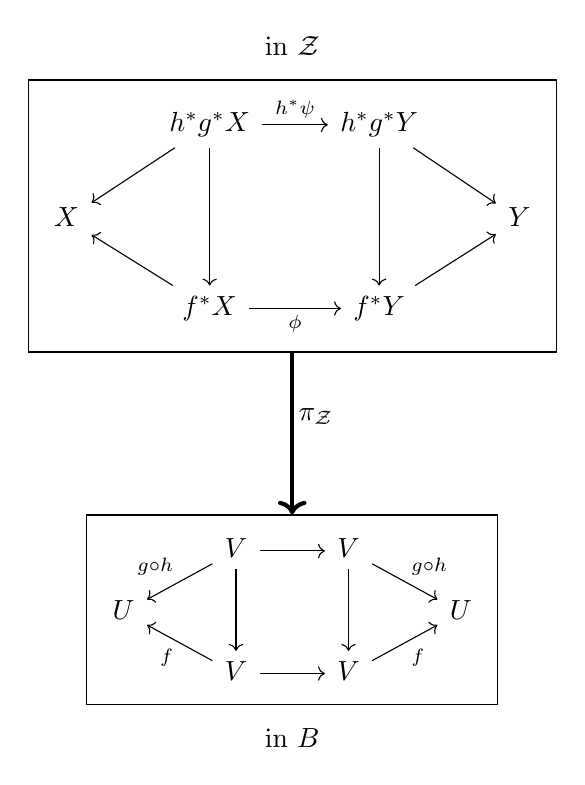
\begin{tikzpicture}[mybox/.style={draw, inner sep=5pt}]
    \node[mybox] (X) at (0,5){%
        \begin{tikzcd}
            {} & h^*g^*X\ar[ld] \ar[r, "h^*\psi"]\ar[dd]& h^*g^*Y \ar[dd]\ar[rd]& {} \\
            X & {} & {} & Y \\
            {} & f^*X\ar[lu]\ar[r, "\phi"']& f^*Y \ar[ru]& {}
        \end{tikzcd}
    };
    \node[mybox] (B) at (0,0){%
        \begin{tikzcd}[row sep=8pt]
            {} & V \ar[ld, "g \circ h"']\ar[r, "\id"]\ar[dd, "\id"']& V \ar[dd, "\id"]\ar[rd, "g \circ h"]& {} \\
            U & {} & {} & U \\
            {} & V \ar[lu, "f"]\ar[r, "\id"']& V \ar[ru, "f"']& {}
        \end{tikzcd}
    };

    \node [above=5pt of X] {in $\stZ$};
    \node [below=5pt of B] {in $\cat{B}$};
    \draw [->, line width=1.5pt] (X) edge (B);
    \node at (0.3,2.45) {$\pi_{\stZ}$};
    \end{tikzpicture}
    \end{center}

    fibrationは次のように与えられる.
    \begin{defmap}
        \pi \colon & \Isom(X, Y)& \to& \cat{B}/U \\
        \textbf{Objects:}& (f \colon V \to U, f^*X, f^*Y, \phi \colon f^*X \to f^*Y)& \mapsto& f \\
        \textbf{Arrows:}& (h \colon V \to W, h^*g^*X \to f^*X, h^*g^*Y \to f^*Y)& \mapsto& h \\
    \end{defmap}
\end{Def}

\begin{Remark}\label{rem:simple_isom}
    $\stX \to \cat{B}$のsplittingを選んだ場合には$\Isom(X, Y)$の定義は次のように簡単に成る.
    \begin{description}[labelindent=1cm]
        \item[Object.]
             $\cat{B}/U$の対象$f \colon V \to U$と同型$\phi \colon f^*X \to f^*Y$の組.

        \item[Arrow.]
            射$(f, \phi) \to (g, \psi)$は,
            $g \circ h=f$を満たす$\cat{B}/U$の射$h$.
    \end{description}
    以下では$\Isom(X, Y)$がalgebraic space(これはsheaf)と
    同型であるかどうかを考えるので,
    こちらの定義だけを覚えていても問題はない.
\end{Remark}

\subsubsection{Propositions}
\begin{Lemma}
    任意の$U \in \cat{B}$と$X, Y \in \stX(U)$について,
    $\Isom(X, Y)$はcategory fibered in sets.
\end{Lemma}
\begin{proof}
    恒等射上の射は恒等射しかないことを確かめれば良い.
    $\Isom(X, Y)$の射の定義から,恒等射上の射は次の形になっている.
    \[ (\id[U], f^*X \to f^*X, f^*Y \to f^*Y) \colon (f, f^*X, f^*Y, \phi) \to (f, f^*X, f^*Y, \psi) \]
    $f^*X \to f^*X, f^*Y \to f^*Y$はTriangle Liftingから得られるcanonicalなものなので,
    恒等射である.
\end{proof}

$\stX$ :: stackの場合は($\stX \to \cat{B}$のsplittingを選べば)$\Isom(X, Y)$はsheafになる.
\begin{Lemma}
    一般のsite :: $\cat{C}$とCFG :: $\stX \to \cat{C}$をとる.
    さらに$\stX$はsplit fibered categoryであるとする.
    以下の二つは互いに同値.
    \begin{enumerate}
        \item $\stX$はprestackである.
        \item 任意の$X, Y \in \stX$について$\Isom(X, Y)$のfiberはsheafである.
    \end{enumerate}
\end{Lemma}
\begin{proof}
    (TODO: 出典)
\end{proof}

\subsubsection{Representability of Diagonal Morphism.}
\begin{Remark}
    以下,scheme $S$を固定し,
    特に断らない限りbig etale site :: $\ET(S)$上のstack in groupoidsのみ考える.
\end{Remark}

\begin{Lemma}
    $\stX$ :: stack in groupoids on $\cat{C}$($=\ET(S)$)とする.
    この時,$\Diag \colon \stX \to \stX \times_{S} \stX$が表現可能であることと,
    任意の$U \in \cat{C}$と任意の$X, Y \in \stX(U)$について
    $\Isom(X, Y)$がalgebraic spaceであることは同値.
\end{Lemma}
%% {{{
\begin{proof}
    $x,y \colon \Sch/U(=U) \to \stX$を,
    $2$-Yoneda Lemmaにより得られる$X, Y \in \stX(U)$に対応する射とする
    \footnote{ 例えば$x$は$f \in \Sch/U$をcartesian lifting $f^*X$へ写す. }.

    以下の図式がpullback diagramであることから分かる.
    \[
    \begin{tikzcd}[row sep=40pt]
        \Isom(X, Y) \ar[r, "\pr_{U}"]\ar[d, "\pr_{\stX}"']& \Sch/U \ar[d, "x \times y"]\\
        \stX \ar[r, "\Diag"'] & \stX \times_{S} \stX
        \ar[from=2-1, to=1-2, shorten >= 20pt, shorten <= 20pt, Rightarrow, "a"]
    \end{tikzcd}
    \]
    任意の射$\Sch/U \to \stX \times \stX$が$x \times y$の形で表されることは,
    $\stX \times \stX$の普遍性から得られる.

    まず,射と自然同型を定義する.
    $\Isom(X, Y)$から伸びる射は次の関手である.
    ただし
    $\xi=(f \colon V \to U, f^*X, f^*Y, \phi \colon f^*X \to f^*Y),
    \eta=(g \colon W \to U, g^*X, g^*Y, \psi \colon g^*X \to f^*Y)$とした.
    \begin{defmap}
        \pr_{U}& \Isom(X,Y)& \to& \Sch/U \\
        \textbf{Objects:}& \xi& \mapsto& f \\
        \textbf{Arrows:}& [\xi \to \eta]& \mapsto& h \\
        \hfill \\
        \pr_{\stX}& \Isom(X, Y)& \to& \stX \\
        \textbf{Objects:}& \xi& \mapsto& f^*X \\
        \textbf{Arrows:}& [\xi \to \eta]& \mapsto& f^*X \to h^*g^*X
    \end{defmap}
    自然同型$a$は次で定める.
    \begin{defmap}
        a_{\xi}\colon & ((x \times y) \pr_{U})(\xi)& \to& (\Diag \pr_{\stX})(\xi) \\
        {}& (f \colon V \to U, f^*X, f^*X, \alpha)& \mapsto& (\id[f^*X], \phi)
    \end{defmap}

    $\Isom(X, Y)$がpullbackであることは,
    $\Isom(X, Y)$が普遍性を持つことを通して確かめる.
    (TODO)
\end{proof}
%% }}}

\subsection{Proof.}
\subsubsection{\tp{$\Diag$}{The Diagonal Morphism} is Representable.}
示した補題から,
任意の$U \in \cat{C}$と任意の$G_U$-torsor :: $\shP_1, \shP_2 \in \stX(U)$について
$\Isom(\shP_1, \shP_2)$がalgebraic spaceであることは同値である.
これは次のようにして自明な場合に帰着できる.

\step{$\shP_1, \shP_2$が自明な場合に帰着させる.}
\begin{Lemma}[\cite{Olsson16} Exc 5.G]\label{lem:F_is_algsp}
    $U$ :: schemeをとる.
    sheaf on $\ET(U)$ :: $\shF$とetale surjective morphism :: $V \to U$に対し,
    $V \times_{U} \shF$がalgebraic spaceならば,$\shF$はalgebraic space.
\end{Lemma}

\begin{Lemma}\label{lem:UIsom}
    $X, Y \in \stX(U)$と$v \colon V \to U$について
    \[ V \times_{U} \Isom(X, Y) \iso \Isom(v^*X, v^*Y). \]
\end{Lemma}

\begin{proof}[(補題\ref{lem:F_is_algsp}の証明)]
    $\shF':=(V \times_{U} \shF) \times_{V} (V \times_{U} \shF)$とおく.

    まずdiagonal morphismの表現可能性を考える.
    pullback lemmaから次が分かる.
    \[
        (V \times_{U} \shF) \times_{V} (V \times_{U} \shF)
        \iso (V \times_{U} \shF) \times_{U} \shF
        \iso V \times_{U} (\shF \times_{U} \shF).
    \]
    このことから,$\Diag \colon \shF \to \shF \times_{U} \shF$を$V \to Y$でpullbackしたものが
    $\Diag' \colon \shF' \to \shF' \times \shF'$だと分かる.

    atlasの存在は次のように分かる.
    $A \to \shF'$を$\shF'$のatlasとする.
    \[
    \begin{tikzcd}
        A \ar[r]& \shF' \ar[r]\ar[d]& \shF \ar[d]\\
        {} & V \ar[r, "\text{etale, surj.}"']& U
    \end{tikzcd}
    \]
    $V \to Y$がetale surjectiveなので$\shF' \to \shF$もetale surjective.
    今$A \to \shF'$がetale surjectiveなので,併せて$A \to \shF$がetale surjectiveと分かる.
\end{proof}

\begin{proof}[(補題\ref{lem:UIsom}の証明)]
    定義を変形するだけである.
    \begin{align*}
        {}& (V \times_{U} (\Isom(X, Y)))(W) \\
        =&  V(W) \times_{U(W)} \Isom(X, Y)(W) \\
        =&  \{ (w \colon W \to V, f \colon W \to U, \rho \colon f^*X \isomap f^*Y) \mid u \circ v=f \} \\
        =&  \{ (w \colon W \to V, \rho \colon w^* u^*X \isomap w^* u^*Y) \} \\
        =&  \Isom(v^*X, v^*Y)(V)
    \end{align*}
\end{proof}

$\shP_1, \shP_2$が自明に成るetale cover :: $\covV$
\footnote{ i.e. $\Forall{V \in \covV} \shP_1(V), \shP_2(V) \neq \emptyset$. }
をとり,$v \colon V=\bigsqcup_{V \in \covV} V \to X$とすれば,
$v^*\shP, v^*\shP_2$は自明な$G_U$-torsorとなる.
こうして$\shP_1, \shP_2$が自明な場合に議論を帰着させることが出来る.

同型$G_Y \iso \shP_1, G_Y \iso \shP_2$を固定する.
これらと$\pi_1, \pi_2$を合成して
\[ \rho_1 \colon G_Y \to X_Y, \quad \rho_2 \colon G_Y \to X_Y \]を得る.

\step{$\shP_1, \shP_2$が自明な場合について証明する.}

$\Isom(\ (G_Y, \rho_1), (G_Y, \rho_2)\ )$がどのようなsheafか考える.
trivial torsorの任意の自己同型$\phi \colon G_Y \to G_Y$は,
これがequivariantであることから,$\phi(e)$の左からの積になっている.
逆に任意の$G_Y$の元を取れば左からの積が自己同型になるから,
集合$\Isom(\ (G_Y, \rho_1), (G_Y, \rho_2)\ )$は$G_Y$の部分集合である.
そこで,$g \in G_Y$ (i.e. $g \colon 1 \to G_Y$)から得られる
自己同型$(\cdot g) \colon G_Y \to G_Y$が満たすべき条件を考える.

$[X/G]$の定義から,次が可換である.
\[
\begin{tikzcd}
    G_Y \ar[rr, "(\cdot g)"]\ar[rd, "\rho_1"']& {} & G_Y \ar[ld, "\rho_2"]\\
    {} & X_Y & {}
\end{tikzcd}
\]
$(\cdot g)$はequivariantだから,この図式が可換であることは$\rho_1(e)=\rho_2(g)$と同値である.
したがって
\begin{align*}
    {}& \Isom(\ (G_Y, \rho_1), (G_Y, \rho_2)\ )(V) \\
    =&  \{ g \in G_Y(V) \mid \rho_1(e)=\rho_2(g) \} \\
    =&  \{ (g, x) \in G_Y(V) \times X_Y(V) \mid  (\rho_1(e), \rho_2(g))=(x, x)  \}
\end{align*}
これは次のように,fiber productで表現出来る.
\[
\begin{tikzcd}
    \Isom(\ (G_Y, \rho_1), (G_Y, \rho_2)\ ) \ar[r]\ar[d]& G_Y \ar[d]\\
    X_Y \ar[r, "\Diag"']& X_Y \times_{Y} X_Y
\end{tikzcd}
\]
射$G_Y \to X_Y \times_{Y} X_Y$は$g \mapsto (\rho_1(e), \rho_2(g))$である.
この図式がpullback diagramであることは
$\Isom(\ (G_Y, \rho_1), (G_Y, \rho_2)\ )$がalgebraic spaceであることを意味している.

\subsubsection{\tp{$[X/G]$}{The Quotient Stack} has an Atlas.}
射$a \colon X \to [X/G]$を
trivial $G_X$-torsor :: $(G_X, m_X) \in [X/G](X)$に
($2$-Yoneda Lemmaによって)対応する射とする.
この射$a$がatlasであることを示す.
$a$がrepresentableであることは$\Diag$がrepresentableであることから分かる.
$a$がsmooth, surjectiveであることを示す.

以下のpullback diagramを考える.
\[
\begin{tikzcd}
    \cat{P} \ar[r]\ar[d]& X \ar[d, "{(G_X, m_X)}"]\\
    Y \ar[r, "{(\shP, \pi)}"']& {[X/G]}
    \ar[from=2-2, to=1-1, phantom, "\text{p.b.}"]
\end{tikzcd}
\]
ただし$Y \to [X/G]$は$a$と同様に$(\shP, \pi) \in [X/G](Y)$に対応する射である.
$\shP$は作用$\alpha \colon G_Y \times \shP \to \shP$を持つとする.

この時,$\cat{P}$はsheafとして$\shP$と同型である.
これは次のように同型が得られる.
まず$\cat{P}(U)$は以下の$3$つの組の集合である.
\begin{itemize}
    \item $x \colon U \to X$,
    \item $y \colon U \to Y$,
    \item $\rho \colon x^*(G_X, m_X) \isomap y^*(\shP, \pi))$.
\end{itemize}
ただし$x,y$について以下が可換.
\[
\begin{tikzcd}
    U \ar[r, "x"]\ar[d, "y"']& X \ar[d]\\
    Y \ar[r]& S
\end{tikzcd}
\]
上のような$x,y$を一つとり,$x_0, y_0$と名前を付ける.
すると$(y_0)^*G_Y=(x_0)^*G_X$となる.
$\cat{P}(U)$の元$(x,y, \rho)$が存在するならば,
$x^*X=y^*X_Y$ゆえに$x,y$は上の可換図式を満たすことに注意せよ.

次のように同型を定める.
\begin{defmap}
    {}&\cat{P}(U)& \to& \shP(U) \\
    {}&(x, y, \rho)& \mapsto& \rho_{U}(e) \\
    {}&(x_0, y_0, (y_0)^*\alpha(-, p))& \mapsfrom& p
\end{defmap}
$(f^*\shP)(U)=\shP(U)$は$f^*$のcolomitを用いた定義から得られる.

最後に$\shP \to Y$がetale surjectiveであることを確かめる.
$\shP(Y_i) \neq \emptyset$となる$Y$のcover :: $\{Y_i \to Y\}$をとる.
$\shP|_{Y_i}$はtrivial torsor :: $G_{Y_i}$と同型となる.
$\pr_{Y_i} \colon G_{Y_i} \to Y_i$はsmooth surjectiveであり,
smooth, surjectiveはどちらもetale local on targetな性質なので,
$\shP \to Y$もetale, surjective.
(ついでに$\shP$ :: algebraic spaceも分かる.)

\printbibliography[title=参考文献]
\end{document}
